\section{A.~~Mode identification}
\makeatletter
\protected@edef\@currentlabel{A}
\label{sec:mode identification}
\makeatother
\renewcommand\thefigure{\thesection A.\arabic{figure}} %To set the Fig numbering to B
\setcounter{figure}{0} 

Currently, for our system, assigning mode frequencies to their respective modes of motion is not possible with complete confidence. Since we have only one detection coil, there is no distinction for different degrees of freedom. Although the magnetic flux couples differently to different modes, we cannot yet use this information to assign which mode is which because we cannot assume that the equilibrium position of the magnet is exactly in the center of the trap.

We find different resonance frequencies between cooldowns without making changes to the setup, or when warming up the trap above the critical temperature of the superconductor and subsequently cooling down again. We attribute this to some flux from the magnet remaining trapped in the superconductor as the superconductor is cooled through its transition from being a normal metal to becoming a superconductor, although the type I superconductor expels most of the magnetic field. We have calculated the expected frequencies for the modes with analytical models~\cite{Vinante2022,Francis2025}.

The order, from low frequency to high frequency, we find from the analytical calculations is always: $\gamma$, z, y, x, $\beta$, $\alpha$ with the axes shown in Fig.~\ref{fig:Magnet axis}. Also when varying the dimensions of the trap slightly around the values of our particular trap, the values for the frequencies change, but the order of frequencies does not change. This means, although not with complete confidence, that the described mode 3 would belong to the y-mode and mode 4 would belong to the x-mode of the particle.

We also varied the inclination angle ($\beta$) of the particle with respect to the horizontal axis. This is done by purposely gluing the glass bead asymmetrically below the magnet, to avoid that one of the modes would couple very weakly to the pick-up coil. However, we don't know at exactly what inclination angle the magnet will levitate in the trap. This also does result in the same order of frequencies.


\begin{figure}[h]
    \centering
    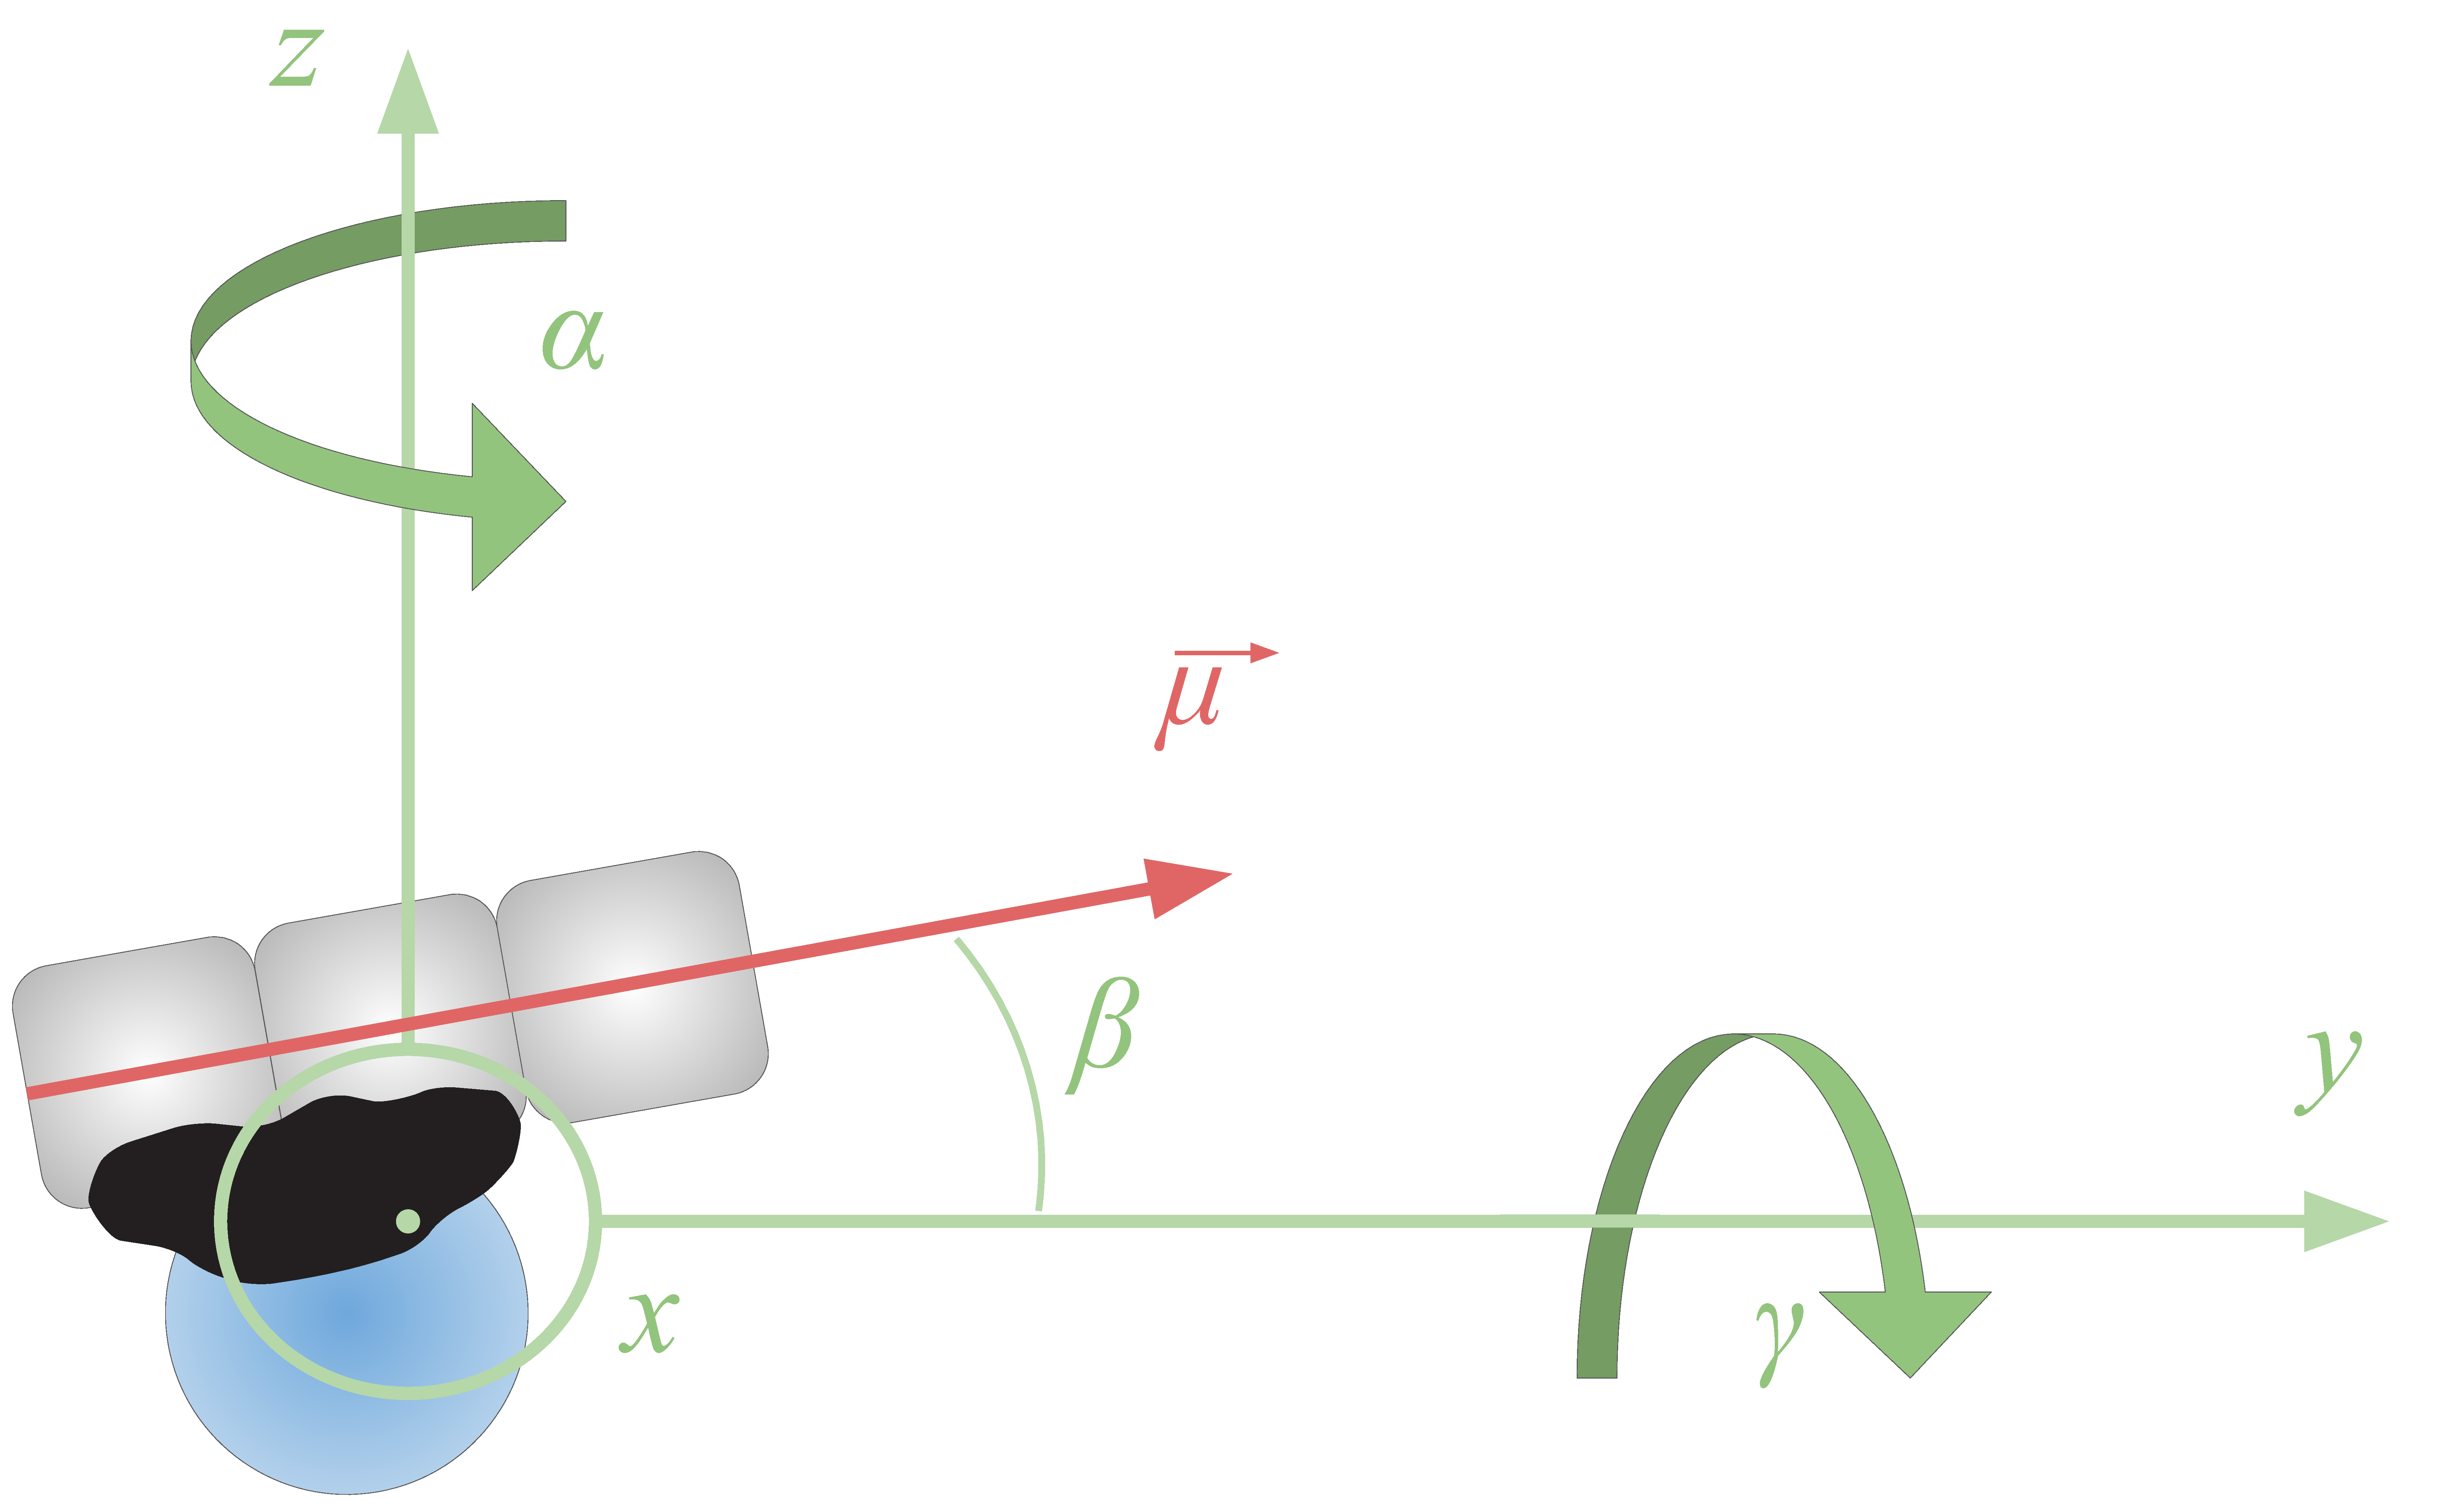
\includegraphics[width=0.63\columnwidth]{5-Appendix/Figures/Magnet_axis.pdf}
    \caption{The defined axes of the levitated magnet.}
    \label{fig:Magnet axis} 
\end{figure}
